% !TeX root = ../main.tex

\chapter{可配置动态图生成组件设计与实现}
\label{cha:chapter03}

在整个动态社交网络图生成管理系统中,可配置动态图生成组件是其中的核心。为了能够生成动态图,我们需要首先实现静态图的生成算法,并且在此基础上加以扩展,实现第\ref{cha:structure_dynamic}节中的动态图事件以体现图的动态性。在算法的设计基础上,生成组件的实现需要进行整体架构设计,也需要考虑动态图存储结构的设计。

生成组件的实现基于第\ref{cha:node_edge_dynamic}节与第\ref{cha:structure_dynamic}节中对图动态性的分析、第\ref{cha:generatorscheme}节展示的动态图生成配置方式,用户定义的配置信息使用JSON格式进行存储与读取。生成组件实现过程中使用的语言是Python,并且在生成过程中使用了numpy库。

\section{静态图生成算法}
\label{cha:staticgraph}

静态图的生成是动态图生成的基础。在给定节点数量、边的度数分布特征(入度分布与出度分布)、社区分布特征之后,即可进行静态图的生成操作。生成过程包括节点度数确定与边的目标节点确定\cite{FastSGG}两部分,分别利用了出度分布与入度分布的信息。在确定每一个节点的出度并且确定每一条边的目标节点后,即可得到一个完整的图。

\subsection{节点度数确定算法}

节点出度确定相对比较简单。在给定出度分布(已经包含所需参数的概率密度函数$dist_{out}$)与最小度数$d_{min}$、最大度数$d_{max}$之后,可以用公式\ref{equ:DegreeDetermine}计算得到每一个可能的度数对应的概率:

\vspace{-8mm}

\begin{equation}
  \label{equ:DegreeDetermine}
  P\left(outd_i=m\right)=\frac{dist_{out}(m)}{\sum\limits_{j=d_{min}}^{d_{max}}dist_{out}(j)}
\end{equation}

在此之后,即可使用得到的概率信息为每个节点随机分配出度。在numpy中提供了一个随机函数np.random.choice可以按照给定的概率随机取值,只需将可用度数列表与计算出的概率信息传入即可随机生成。

用公式\ref{equ:DegreeDetermine}确定每个度数对应概率、选择每个节点的出度的具体过程如算法\ref{alg:DegreeDetermine}所示,其中包含每一个度数对应概率的计算、归一化、度数选择几个部分。

% \lstinputlisting[
%     style       =   Python,
%     caption     =   {\bf Degree Determine},
%     label       =   {degree.py}
% ]{code/degree.py}

\begin{algorithm}[htb]
  \caption{确定每个节点出度的算法}
  \label{alg:DegreeDetermine}
  \begin{algorithmic}[1]
    \Require
      出度分布的概率密度函数$dist_{out}$,
      出度分布最小度数$d_{min}$,
      出度分布最大度数$d_{max}$
    \Ensure 某个节点的出度
    \Function {DegreeProb}{$dist_{out}, d_{min}, d_{max}$}
      \State $P \gets []$
      \State $sum \gets 0$
      \For{each $i\in [d_{min}, d_{max}]$}
        \State $P[i - d_{min}] \gets dist_{out}(i)$
        \State $sum \gets sum + P[i - d_{min}]$
      \EndFor
      \For{each $i\in [d_{min}, d_{max}]$}
        \State $P[i - d_{min}] \gets P[i - d_{min}] / sum$
      \EndFor
      \State \Return $P$ // 每一个度数对应的概率$P$(列表形式,第一个元素对应于$d_{min}$)
    \EndFunction
    \State $P \gets$ DegreeProb$(dist_{out}, d_{min}, d_{max})$
    \Function {GetOutDegree}{$d_{min}, d_{max}$}
      \State \Return $choice([d_{min}, d_{max}], P)$
    \EndFunction
  \end{algorithmic}
\end{algorithm}

\subsection{边的目标节点确定算法}
\label{cha:DetermineTarget}

上一节中可以通过得到的概率信息用随机方法给每一个节点分配其出度,也就是确定了以该节点为起点的边的数量。在此基础上,需要确定每一条边对应的目标节点。为了能够更清晰地解释目标节点确定算法,使用例\ref{exa:choose_t_graph}对算法思想进行说明,在此之后将给出具体的算法流程。

\begin{example}
  \label{exa:choose_t_graph}
  参数为$1.12$的power-law分布,节点总数$100$,度数范围$[1, 10]$
  
  将所有节点按照入度从小到大排序,只需选择最后的节点排序序号即可进行目标节点的选择。

  对度数为$i$的节点进行分析,存在归一化参数$\alpha, \beta$使得:
  
  \begin{itemize}
    \item 入度为$i$的节点占所有节点的比例为:$\alpha \times i^{-1.12}$
    \item 目标节点的入度为$i$的边占所有边的比例为:$\beta \times i \times \alpha \times i^{-1.12}$
  \end{itemize}

\vspace{0.2cm}

  \begin{figure}
    \centering
    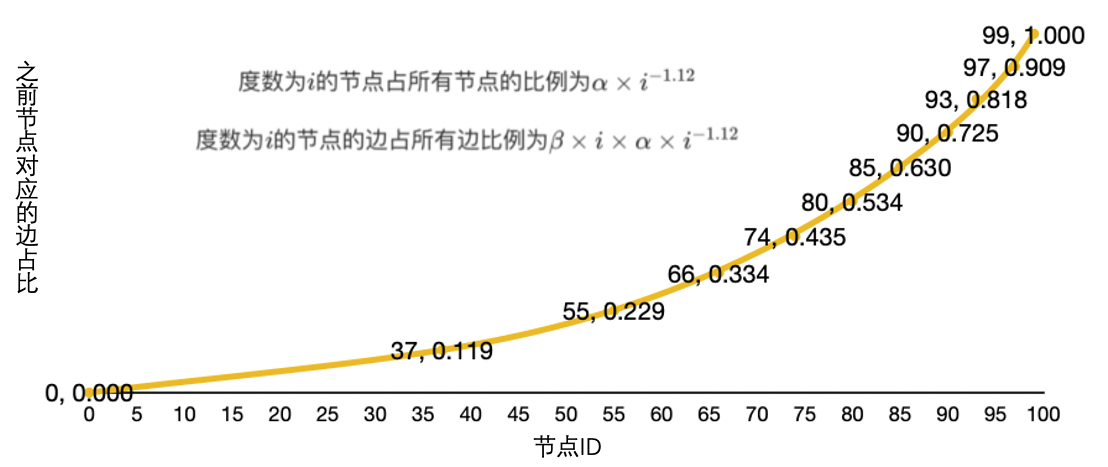
\includegraphics[scale=0.3]{choose_t1.png}
    \caption{示例-一个Power-Law分布节点选择过程1}
    \label{fig:target_node_choose1}
  \end{figure}
  
  如图\ref{fig:target_node_choose1}所示,图中标出的节点横纵坐标其实是累积量,如$55, 0.229$点表示入度不超过$2$的节点一共有$55$个,并且以这些节点为目标节点的边占比为$22.9\%$:
  
  \begin{itemize}
    \item 横坐标:入度不超过$m$的节点个数:$100 \times \sum\limits_{i = 1}^{i <= m} \alpha \times i^{-1.12}$
    \item 纵坐标:目标节点入度不超过$m$的边占比:$\sum\limits_{i = 1}^{i <= m} \beta \times i \times \alpha \times i^{-1.12}$
  \end{itemize}

\vspace{0.2cm}

  由于图中纵坐标表示的是边的累计分布。因此在选择目标节点时,可以在$[0, 1)$区间内得到一个随机数$r$,找到纵坐标为$r$对应点的横坐标,即为需要的节点序号。这一过程可以分为两步:确认入度范围、在范围中取值找到目标节点序号。

  \begin{figure}
    \centering
    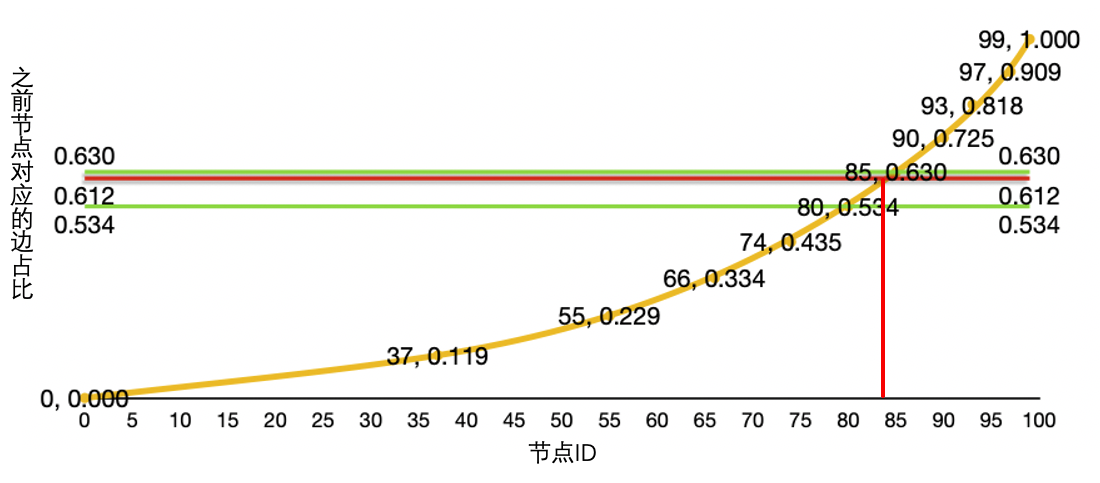
\includegraphics[scale=0.3]{choose_t2.png}
    \caption{示例-一个Power-Law分布节点选择过程2}
    \label{fig:target_node_choose2}
  \end{figure}
  
  如图\ref{fig:target_node_choose2}所示,当随机数选择为$0.612$时,确定横坐标的过程可以为:

  \begin{itemize}
    \item 确认$0.612$对应的点所在区间:从图\ref{fig:target_node_choose2}上可以看到$0.534<0.612<0.630$,两个定位点分别是$80, 0.534$和$85, 0.630$,所以应当在入度为$6$的节点中选择
    \item 目标节点序号取为:$80+\frac{0.612-0.534}{0.630-0.534} \times(85-80) \approx 84$
  \end{itemize}
\end{example}

通过对例\ref{exa:choose_t_graph}的讨论,可以得到目标节点选择算法的一个直观理解。接下来,将对例子中涉及到的公式进行重新定义,并且给出一个完整的选择算法。

% 但是上述算法存在一些问题:

% \begin{itemize}
%   \item 在给定随机数之后找到这个纵坐标对应的点需要用遍历或二分查找的方法,在度数范围比较大的情况下可能需要较长时间。
%   \item 节点个数变化时需要重新计算对应的横坐标。
% \end{itemize}

第一步是为所有节点分配一个重要性排序,排序在前的节点重要性较低,即排序在前的节点入度相对较小。

用公式\ref{equ:NodeInDegreeDetermine}即可确定每一个入度的节点在所有节点中占的比例,进而用累积的方法即可得到在节点排序中的区间:

\vspace{-8mm}

\begin{equation}
  \label{equ:NodeInDegreeDetermine}
  P\left(ind_i=m\right)=\frac{dist_{in}(m)}{\sum\limits_{j=d_{min}}^{d_{max}}dist_{in}(j)}
\end{equation}

确定一条边的目标节点时,需要按照公式\ref{equ:TargetProb}计算目标节点的入度为$m$的概率:

\vspace{-8mm}

\begin{equation}
  \label{equ:TargetProb}
  P\left(ind_{edge_i}=m\right)=\frac{dist_{in}(m) \times m}{\sum\limits_{j=d_{min}}^{d_{max}}dist_{in}(j)\times j}
\end{equation}

这里需要特别注意,在公式\ref{equ:NodeInDegreeDetermine}和公式\ref{equ:TargetProb}中,分别计算的是\textbf{所有节点中入度为$m$的概率}和\textbf{所有边中目标节点的入度为$m$的概率},因此其表示形式不同。

基于前述讨论,边的目标节点选择过程包含以下几步:

\begin{enumerate}
  \item 确定每个节点的排序信息,可以使用一个随机打乱函数实现,排序在前的节点入度较低;
  \item 依据公式\ref{equ:NodeInDegreeDetermine},按照排序信息确定每个度数对应的节点范围;
  \item 依据公式\ref{equ:TargetProb},计算该边选择目标节点度数为$i$的概率$P$;
  \item 按照得到的概率$P$,随机选择每一条边目标节点对应的入度;
  \item 得到入度后,在这个入度对应的节点范围中进行随机选择。
\end{enumerate}

\vspace{0.2cm}

在例\ref{exa:choose_t}中给出了一个计算公式\ref{equ:NodeInDegreeDetermine}和公式\ref{equ:TargetProb}两个概率的示例。

\begin{example}
  \label{exa:choose_t}
  两个概率的计算\\
  \textbf{条件:}节点个数为2,入度范围为$[1,2]$,对应的概率密度函数为:$P(ind_i=1)=0.4, P(ind_i=2)=0.6$,节点排序为[1,0](即:下标为0的节点代表2号节点)\\
  \textbf{计算过程:}
  \begin{itemize}
    \item 所有节点中入度为1的概率为0.4,入度为2的概率为0.6
    \item 节点$[0, 0.8)$对应的入度分配为1,节点$[0.8,2]$的入度分配为2\footnote{注意这里的节点范围是浮点数而非整数。如果后续确定应该在入度为2的节点中选择,则会在$[0.8,2]$范围内均匀取随机数取整得到结果,即所得结果在$[0.8,1)$范围内则目标节点为排序中下标为0的节点。同时,也可以直接对每个入度对应的节点范围取整处理而非使用浮点数。}
    \item 选择的目标节点入度为1的节点的概率为$\frac {0.4\times 1}{0.4\times 1 + 0.6\times 2}=0.25$
    \item 选择的目标节点下标为0(2号)的概率为$0.25 + (1-0.25)\times\frac{1-0.8}{2-0.8}=0.375$
  \end{itemize}
\end{example}

进行目标节点选择的完整算法如算法\ref{alg:TargetNodeProb}所示。

\begin{algorithm}[htb]
  \caption{确定一条边的目标节点}
  \label{alg:TargetNodeProb}
  \begin{algorithmic}[1]
    \Require
      入度分布的概率密度函数$dist_{in}$,
      入度分布最小度数$d_{min}$,
      入度分布最大度数$d_{max}$,节点排序数组$Nodes$
    \Ensure 某条边的目标节点
    \Function {EdgeDegreeProb}{$dist_{in}, d_{min}, d_{max}$}
      \State $P \gets []$
      \State $sum \gets 0$
      \For{each $i\in [d_{min}, d_{max}]$}
        \State $P[i - d_{min}] \gets dist_{in}(i) \times i$
        \State $sum \gets sum + P[i - d_{min}]$
      \EndFor
      \For{each $i\in [d_{min}, d_{max}]$}
        \State $P[i - d_{min}] \gets P[i - d_{min}] / sum$
      \EndFor
      \State \Return $P$ // 每一个度数对应的概率$P$(列表形式,第一个元素对应于$d_{min}$)
    \EndFunction
    \State $P \gets$ DegreeProb$(dist_{in}, d_{min}, d_{max})$ // 可以直接调用确定出度概率的函数
    \State $P_{edge} \gets$ EdgeDegreeProb$(dist_{in}, d_{min}, d_{max})$
    \Function {GetTargetNode}{$d_{min}, d_{max}$}
      \State $degree \gets choice([d_{min}, d_{max}], P_{edge})$
      \State $node \gets choice(P[degree])$
      \State \Return $Nodes(int(node))$
    \EndFunction
  \end{algorithmic}
\end{algorithm}

\subsection{社区处理}
\label{cha:Community}

社区的划分从本质上看就是将所有节点分类,可将每个社区的节点ID放在一个集合中进行存储。实现时由用户在配置信息中指定各个社区的规模之比,用随机的方法进行节点所属社区的分配。

在\ref{cap:simplegen}节中曾给出了社区参数$\rho$的定义,表示社区间生成边的概率与社区内部生成边的概率的比值。为了生成能够满足社区结构的图,可以对于生成的每一条边进行检测,得到的结果如果不在同一个社区内则按照概率$1-\rho$进行舍弃。这样得到的图即可满足社区参数$\rho$的要求。

\section{动态图事件处理}
\label{cha:Dynamic_deal}

第\ref{cha:staticgraph}节对生成静态图的方法进行了探讨,给出了对应的伪代码。而为了生成动态图,需要基于上述过程进行扩展,加入在第\ref{cha:chapter02}章讨论的动态特性。

在表\ref{tab:events}中已经定义了多种动态图事件,在此将介绍其具体实现,包括:

\begin{itemize}
  \item 节点个数的变化
  \item 边个数的变化
  \item 节点在分布中的重要度变化
  \item 社区参数的变化
\end{itemize}

\vspace{0.2cm}

在进行事件具体的实现之前,首先对需要记录的数据类型进行分析。除了节点、边、社区信息需要存储之外,节点在分布中的重要度信息也是必不可少的。

\subsection{节点映射}
\label{cha:node_map}

在出度确定与边的目标节点确定过程中,都会体现出节点度数的不同,而这也就体现了不同节点的重要程度。同时,许多动态图事件也与节点重要度的变化有关。为了解决这一问题,本节提出了一种叫做“节点映射”的结构,用此结构进行节点重要度信息的存储。

节点映射包括两部分:

\begin{itemize}
  \item 出度分布:进行出度的分配后,得到的结果代表了节点的重要程度。因此,对于出度分布而言,可以直接使用初次分配得到的节点出度信息。
  \item 入度分布:第\ref{cha:DetermineTarget}节中曾经说明节点排序信息在目标节点选择算法中的应用,入度分布节点映射即为对节点重要程度的表征。
\end{itemize}

\vspace{0.2cm}

形式上来说,节点映射的形式为:

\begin{itemize}
  \item 出度分布:节点ID到节点出度的字典。
  \item 入度分布:排序\footnote{排序在前的节点ID重要性较低,入度较小}后,节点ID组成的数组。
\end{itemize}

\vspace{0.2cm}

出度分布节点映射中的信息可以指导后续的生成过程。也就是说,对于初始重要度比较高(选定的出度更大)的节点,后续生成过程中的出度往往也会更大。入度分布节点映射则可以直接影响边目标节点的选择,在入度分布的节点映射不变的情况下,节点相对的重要程度在后续生成过程中也不会改变。

\subsection{事件的实现方式}

本节将对各种事件的具体实现方式进行介绍。由于事件中需要确定每个事件发生、结束的时刻,因此本节引入了“帧”的概念。一帧代表一个时刻,对应于动态图中保存的一个快照。同时,配置时需要提供动态图中涉及到的总帧数(动态图存储的快照数目,即时间序列的长度),以便在后续的生成过程中使用。

\subsubsection{边的生成}

在动态图的生成过程中,边的生成是里面非常重要的一部分。一种比较简单的生成方式是:

\begin{enumerate}
  \item 根据给定的节点配置、边的出度分布信息,计算出每一个节点的出度;
  \item 根据给定的帧数进行分配,计算得到该帧需要生成的边个数。这一过程中可以在平均分配的基础上加入随机因素;
  \item 根据得到的该帧边数目进行生成操作。
\end{enumerate}

\vspace{0.2cm}

\subsubsection{节点新增}

在新增节点后需要重新调整节点映射,其中的关键在于原有节点重要性信息的保持。对于出度分布而言,在不改变原有节点出度的基础上计算新的节点出度即可。但是对于入度分布,需要考虑原有节点在所有节点中相对位置,可以用等比例缩放的方法。具体可以用式\ref{equ:newpos}表示,其中$N_{old}, N_{new}$分别表示新增节点前后的节点总数,$pos, pos_{new}$则分别表示在新增节点事件之前与之后某原始节点的位置(用数组下标表示):

\vspace{-8mm}

\begin{equation}
  \label{equ:newpos}
  pos_{new} = \text{int}\left(pos\times \frac{N_{new}}{N_{old}}\right)
\end{equation}

将原有节点的位置等比例缩放后剩余的空间将随机填入新增的节点。例如,在原有节点个数为3、入度分布节点映射为$[1,2,0]$的情况下,新增7个节点之后原有的节点ID将被调整到如下位置:$[1,\_,\_,2,\_,\_,0,\_,\_,\_]$,空余位置会将新节点调整顺序之后排入。

在节点新增时还需考虑新节点所属社区。在此可以采用随机的方式,为新增节点根据不同社区的规模按照对应比例进行社区分配。

\subsubsection{边与节点删除}

边的删除较为简单,直接从记录中按照要求去掉对应比例边即可。节点删除会导致其关联的边删除,并且节点映射等结构也会随之受到影响。

对于节点的删除事件,在一些真实社交网络上并不多(相对于节点新增而言),如在微博上关注关系图中用户被官方封号、引文网络某篇文章被撤稿,在这两个社交网络中节点删除的操作并不多。

为了尽量减少总的运算量,可以采用集合的方式记录被删除的节点,在新的生成过程中遇到这个节点后跳过即可。

在实现过程中可以设置一个阈值$\alpha$,若删除节点数与总节点数的比值低于$\alpha$则使用前述集合记录被删除节点的方式,反之则进行节点映射的调整,具体操作同节点新增操作。

\subsubsection{社区结构变化}

在日常生活中经常可以看到不同社区之间融合、小团体的形成等现象,这些对应于社区结构的变化。这些变化包括社区参数$\rho$的变化、社区的融合与分裂。

在\ref{cha:Community}节中介绍了社区的应用方式,社区结构可以用一个字典形式进行存储,对社区结构的改变与参数$\rho$的改变只作用于后续新生成的边,新生成的边按照新的社区划分与参数$\rho$进行一定概率的舍弃操作即可。

\subsubsection{节点重要度改变}

在表\ref{tab:events}中,定义了两个与节点重要度改变有关的事件,分别是“突发事件”与“节点重要度变化”,前者是聚焦于突发事件导致的节点重要度的临时性改变,而后者则着重强调节点重要度的永久性改变。临时性改变是可逆的,因此需要保存改变的记录,以便后续恢复。

在节点重要度变化的过程中,修改的其实就是分布对应的节点映射。因此,需要分出度分布和入度分布分别讨论:

\begin{itemize}
  \item 出度分布节点映射:可以将其中某个节点的出度提高,或者将两个节点的出度互换;
  \item 入度分布节点映射:将两个节点的位置互换即可。
\end{itemize}

\vspace{0.2cm}

\section{可配置动态图生成组件的实现}
\label{cha:tool_implementation}

在前两节进行了动态图生成算法的介绍,具体实现时则较为复杂,还考虑配置解析、整体架构、存储方式等内容,在此节中将会对这些内容进行介绍。

\subsection{整体架构}

生成组件时的整体架构如图\ref{fig:structure}所示,具体介绍如表\ref{tab:dyn_stru}所示。

\begin{table}[htb]
  \centering
  \caption[动态社交网络图生成整体架构]{动态社交网络图生成整体架构}
  \label{tab:dyn_stru}
  \begin{minipage}[t]{1\textwidth}
    \begin{tabularx}{\linewidth}{llX}
      \toprule[1.5pt]
      {\heiti 层级} & {\heiti 名称} & {\heiti 说明} \\
      \midrule[1pt]
      解析层 & 配置解析器 & 相关配置的输入与解析 \\\hline
      调度层 & 调度管理器 & 接收解析部分得到的配置信息,进行任务安排、相关内容的存储 \\\cline{2-3}
       & 事件列表 & 解析与存储用户定义的各类事件 \\\cline{2-3}
       & 任务列表 & 将图的生成与各种事件抽象为“任务”这一概念,每一个任务可能由几个步骤组成 \\\cline{2-3}
       & 行为列表 & 将任务进行后续处理,其中对结构有影响的基本步骤被称为“行为”(如:修改某个边对应分布的节点映射,修改某个边对应社区的参数) \\\cline{2-3}
       & 节点信息 & 节点标签、数量、属性,事件中被删除、禁用的节点列表等 \\\cline{2-3}
       & 边信息 & 边的标签、属性、社区配置、分布信息、节点映射等 \\\cline{2-3}
       & 存储信息 & 存储格式、所在目录等 \\\hline
      生成层 & 事件执行器 & 根据指令执行各事件对应的行为,可能修改动态图结构特征 \\\cline{2-3}
       & 生成管理器 & 调用事件执行器进行相应事件的执行,并且进行生成操作,将每一帧生成的结果送入存储管理器中保存 \\\cline{2-3}
       & 存储管理器 & 以指定格式在指定位置存储生成结果 \\
      \bottomrule[1.5pt]
    \end{tabularx}
  \end{minipage}
\end{table}

% \begin{itemize}
%   \item 解析部分:相关配置的输入与解析,进行调度与生成工具的配置与初始化;
%   \item 调度与生成工具部分:接收解析部分得到的配置信息,进行任务安排、相关内容的存储,包含以下部分:
%   \begin{itemize}
%     \item 任务列表生成:将图的生成与各种事件抽象为“任务”这一概念,每一个任务可能由几个步骤组成;
%     \item 行为列表生成:将之前得到的任务进行后续处理,其中对结构影响的基本步骤被称为“行为”(如:修改某个边对应分布的节点映射,修改某个边对应社区的参数);
%     \item 调度器:维护一个时钟,每一帧都检查该帧需要执行的基本步骤(即上文的“行为”),进行对应函数的调用;
%     \item 结构信息存储:存储在生成过程中需要的各种信息,包括:
%     \begin{itemize}
%       \item 节点标签、数量、属性,事件中被删除、禁用的节点列表等;
%       \item 存储相关的文件句柄、目录管理、已生成边和节点的记录等;
%       \item 边的标签、属性、社区配置、分布配置、节点映射等。
%     \end{itemize}
%   \end{itemize}
% \end{itemize}

解析层负责进行配置解析,用户自定义的配置信息在第\ref{cha:generatorscheme}节中有详细介绍,格式如表\ref{tab:dynamic_define}所示,主要包括节点、边、社区、事件这几部分内容,还可以指定存储格式与位置。通过这些信息,可以调度层中所示的事件列表、节点、边、存储的信息这些内容。其中事件列表会进行后续解析,得到每一个事件对应的任务,进一步拆解成一些行为序列(行为是指对结构有影响的基本的操作单元,如修改某个边对应社区的参数,一个任务中可能包括多个行为)。

\begin{figure}
  \centering
  
\includegraphics[scale=0.6]{structure_new.png}
  \caption{动态社交网络图生成整体架构}
  \label{fig:structure}
\end{figure}

接下来将由调度管理器进行管理,每一帧都调用对应的生成任务并进行事件的执行,每一帧的结果会送入存储管理器以给定格式在给定位置进行存储。

\subsection{结果保存}

\begin{table}[htb]
  \centering
  \caption[图存储结构]{生成的动态图存储结构}
  \label{tab:store}
  \begin{minipage}[t]{1\textwidth}
    \begin{tabularx}{\linewidth}{llXX}
      \toprule[1.5pt]
      {\heiti 分类} & {\heiti 名称} & {\heiti 说明} & {\heiti 示例(之前已有$0\rightarrow 1$,此帧新增$0\rightarrow 2, 1\rightarrow 2, 2\rightarrow 0$)} \\
      \midrule[1pt]
      快照形式$^{*}$ & TSV & 文本格式,每行记录一条边 & \tabincell{l}{0 1\\0 2\\1 2\\2 0} \\\cline{2-4}
       & ADJ & 文本格式,每行记录起始节点与对应的边 & \tabincell{l}{0 1 2\\1 2\\2 0} \\\cline{2-4}
       & CSR & 正向表,第一个文件记录节点后继的位置,第二个文件记录所有后继节点 & \tabincell{l}{第一个文件:0 2 3\\第二个文件:1 2 2 0} \\\cline{2-4}
       & Neo4j & 在Neo4j数据库中进行存储,以属性形式存储帧数信息,可以限定帧数进行查询 & 略 \\\cline{2-4}
       & node\_link & JSON格式存储、记录每一个节点、每一条边的信息 & \tabincell{l}{\{``directed": True,\\\ \ ``multigraph": False,\\\ \ ``graph": \{\},\\\ \ ``nodes": [\{``id": 0\},\\\ \ \ \ \{``id": 1\}, \{``id": 2\}],\\\ \ ``links": [\\\ \ \ \ \{``source": 0, ``target": 1\},\\\ \ \ \ \{``source": 0, ``target": 2\},\\\ \ \ \ \{``source": 1, ``target": 2\},\\\ \ \ \ \{``source": 2, ``target": 0\}]\}} \\\hline
      增量形式 & DIFF & JSON格式存储增加与删除的边、增加与删除的节点 & \tabincell{l}{\{``nodes\_added": [2],\\\ \ ``nodes\_deleted": [],\\\ \ ``edges\_added": [(0, 2), \\\ \ \ \ (1, 2), (2, 0)],\\\ \ ``edges\_deleted": []\}}\\
      \bottomrule[1.5pt]
    \end{tabularx}\\[2pt]
    \footnotesize *:直接将每一帧的数据保存到一个文件中,以文件命名区分帧数
  \end{minipage}
\end{table}

本节将介绍动态图生成组件实现的一部分可用存储结构,并且用示例加以说明,具体如表\ref{tab:store}所示。其中列出的格式可以分成快照形式(每一帧的数据单独存储)与增量形式(记录每一帧与之前一帧的区别,以达到节省存储空间的目的)两类,其中增量形式所记录的新增的边、删除的边等内容也可以用与快照形式中相同的方法存储。

除了表\ref{tab:store}中呈现的格式,还实现了networkx中支持的GraphML、ADJACENCY、CYTOSCAPE、JIT等格式,并且可以很方便地修改支持其他格式。

\section{本章小结}

本章对动态图的生成算法进行了详细介绍,并且对动态图生成系统中生成组件的实现细节进行了讨论。第\ref{cha:staticgraph}节与第\ref{cha:Dynamic_deal}节专注于算法与原理方面,在第\ref{cha:tool_implementation}节中主要介绍了生成组件整体架构与结果存储方式等组件实现方面的内容。